\section{Planning with learned model}

In this section two architectures are described. Both involve a similar model learning approach, but differ substantially in technical details and planning algorithms. Nevertheless, the goal stays the same: train a sufficient environment model, or such that accurately predicts future latent states of an environment to predefined cut-off point in time, and use it to plan and solve the environment. The more accurate the model to the cut-off point, which might be environment dependent, the better model learning algorithm.
Before all of that, the code architecture and the framework that was created to accelerate this research are described.

\editnote{NOTE! Related work described those methods in details. Here you need to describe how YOU use them!}

\subsection{HumbleRL framework}

\begin{enumerate}
\item Framework description.
\item Implementation architecture.\\ Note it is used in World Models + AlphaZero.
  \begin{enumerate}
  \item OpenAI Gym is an environment.
  \item Vision is an interpreter.
  \item Memory is a MDP.
  \item AlphaZero is a mind that uses MDP to construct search tree.
  \item Callbacks are used to collect data and statistics.
  \end{enumerate}
\item Copy and adjust diagrams from HRL paper.
\end{enumerate}

\subsubsection{Framework description}
Reinforcement Learning scientists tend to write the entire code from scratch by themselves, instead of using existing RL frameworks. This is justified by the fact, that the commonly available frameworks are not flexible enough for intended experiments or require a specific backend like TensorFlow, which might be disfavored.
HumbleRL \cite{Code.HRL} was created with this problem in mind. Its simple API allows to perform a variety of RL experiments without any restrictions on the algorithms used. Since the backend is not tied to any specific technology, it is possible to mix different neural network frameworks or not use any at all. HumbleRL provides the boilerplate code of RL loop in fig.\ref{Fig.RL} and determines the common interface, the rest is done by the user.

\subsubsection{Implementation architecture (World Models + AlphaZero)}
We show framework architecture in fig. \ref{Fig.HRL_architecture}. An agent is represented by the Mind class. Mind encapsulates action planning logic and provides it via the plan method. In order to learn, the agent acts in the world represented by the Environment class. The Environment class provides methods for resetting, taking steps, rendering and getting information about the world. The agent isn’t usually presented with raw environment observations - instead, it looks at states preprocessed by the Interpreter. Different interpreters can be joined together with the ChainInterpreter class. It acts as a preprocessing pipeline, with each subsequent interpreter using the output of a previous one as an input.
Framework user doesn’t need to call all of those methods directly, those are utilized by the loop function. This function gets an action from the Mind, executes it in the Environment and then next observation is preprocessed with the Interpreter in preparation for the next step. To extend basic loop functionality, user can define callbacks that implement the Callback interface. Callbacks can react to events:
• at the beginning and ending of the loop,
• at the beginning and ending of each episode, • after action is planned by the Mind,
• after step is taken in the Environment.
Callbacks are accumulated in the CallbackList. The entire loop function logic is shown in fig. \ref{Fig.HRL_loop}.
Parallel version of loop function is available as the pool function. It uses predefined number of workers to execute a pool of Minds in their own Environments in parallel.

\begin{figure}[H]
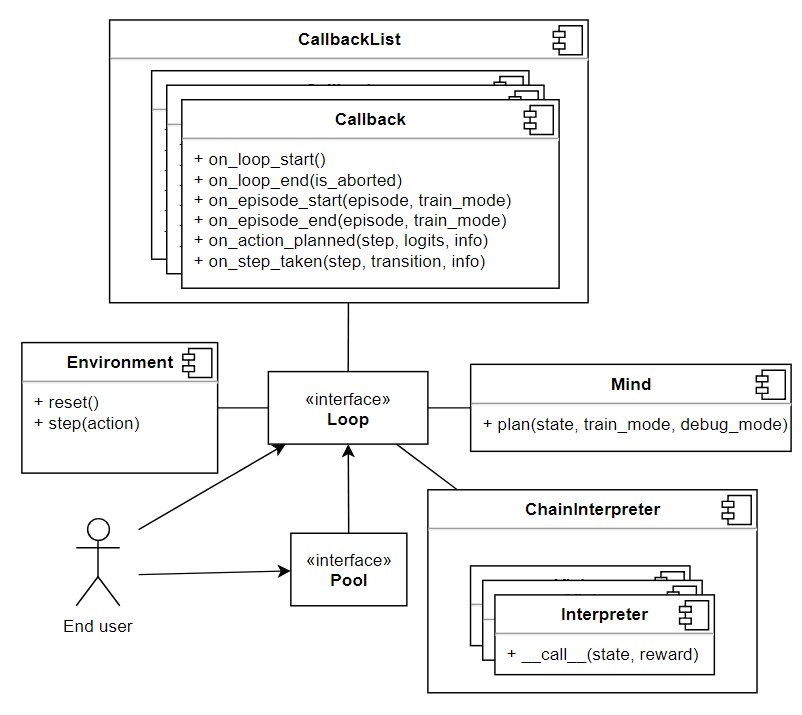
\includegraphics[width=0.45\textwidth,height=0.9\textheight,keepaspectratio]{figures/HumbleRL/architecture.png}
\caption{HumbleRL architecture}
\label{Fig.HRL_architecture}
\end{figure}

\begin{figure}[H]
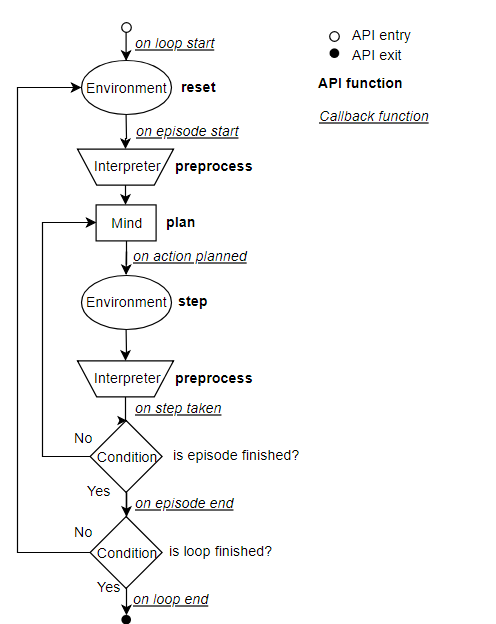
\includegraphics[width=0.45\textwidth,height=0.9\textheight,keepaspectratio]{figures/HumbleRL/loop.png}
\caption{HumbleRL loop function overview}
\label{Fig.HRL_loop}
\end{figure}

\subsection{World Models with the AlphaZero planner}

\begin{enumerate}
\item High-level idea and argument ``why?!'':\\
  World Models shown it can plan (offline planning, training a policy) in imagination and AlphaZero is incredibly powerful search algorithm.
\item Data collection i.e. a random agent.
\item Preprocessing.
\item World Models architecture: Vision and Memory.
  \begin{enumerate}
  \item Which does what (brief reminder) e.g. Vision encode a current observation and Memory encodes history and predicts future.
  \item How Memory is used to predict future: MDN and LMH.
  \item Training procedure of each module i.e. in separation exactly like described in the related work (don't describe loss etc. only high-level).
  \end{enumerate}
\item AlphaZero architecture: Controller.
  \begin{enumerate}
  \item What it does i.e. uses the memory module to plan in imagination.
  \item How next action is planned i.e. MCTS.
  \item Training procedure of Value and Policy networks i.e. policy iteration after Vision and Memory are already trained (don't go into AZ details, it's already in the related work, here how you modify it or apply to your case).
  \end{enumerate}
\end{enumerate}

\subsubsection{High-level idea and argument ``why?!''}
World Models' agent, as shown in the paper\cite{Algo.WorldModels}, is able to learn from simulated experience. It is an example of successful planning using learned model. This work utilize the world model part of the agent in order to learn model of the two mentioned benchmarks. Also, Vision and Memory encode environment observations into low level representation. The latent state of the world models encodes abstract information about the environment and allow the planning controller to stay small.

\subsubsection{Data collection i.e. a random agent.}
To train our V model, we first collect a dataset of 10,000 random rollouts of the environment. We have first an agent acting randomly to explore the environment multiple times, and record the random actions at taken and the resulting observations from the environment. We use this dataset to train V to learn a latent space of each frame observed. We train our VAE to encode each frame into low dimensional latent vector z by minimizing the difference between a given frame and the reconstructed version of the frame produced by the decoder from z.
We can now use our trained V model to pre-process each frame at time t into zt to train our M model. Using this pre-processed data, along with the recorded random actions at taken, our MDN-RNN can now be trained to model P(zt+1 | at, zt, ht) as a mixture of Gaussians.

\subsubsection{Preprocessing.}
Crop middle of the frame and resize (64 x 64 x 3).
Actions one-hot.

\subsubsection{World Models architecture: Vision and Memory.}
We used OpenAI Gym’s CarRacing environment (the same as in original World Models paper), which is a continuous-control, top-down racing environment. The agent receives state pixels as input and controls the break, accelerator and the steering wheel of a car.
We use HumbleRL in a few stages of training the model. First, we use loop together with an agent performing random actions (Mind) and a Callback, that gathers transitions and saves them to an external storage (HDF5 file in our case). The framework allows us to focus strictly on collecting trajectories and not worry about agent-environment interactions.
Transitions are used to train the Vision and Memory components. For Vision, which function is to encode observations into latent state-space, we use Keras and for Memory, which function is to encode history, we use PyTorch [16], since we found it easier to use for this case than Keras. HumbleRL is not constricted to work with any particular deep learning library, so it’s not a problem to mix the solutions, as long as we wrap our trained models in proper interfaces.

\editnote{TODO: Recreate prob. model diagram from your WM vs. PlaNet comparison notes in Draw.io.}
\editnote{TODO: Describe this diagram in probabilistic notation (see note).}

Because Sokoban is the deterministic environment, each experiment with World Models tested also the memory module without Mixture Density Network on top of a RNN. Instead a linear model was used to output the next latent state.
\editnote{TODO: Describe how sampling is done.}

\subsubsection{AlphaZero architecture: Controller.}
Once we have these components ready, we use them to train the final piece - the Controller, which uses Vision and Memory as ChainInterpreter and AlphaZero as Mind. \editnote{TODO: Expand with 1/2 sentences on usage of Vision/Memory.}
We took already implemented board games [13] and wrapped each in the MDP class to represent them as Markov Decision Processes [14] (MDP). MDP is used for MCTS simulations, but also as the Environment. The Mind class implements MCTS algorithm for one player. In AlphaZero, it uses the DNN to evaluate each node and guide search direction on each edge. We compose two Minds in AdversarialMind class that choose which player should take action based on a current state. In the Interpreter class, we take care of states normalization. Each player always sees the board as if he’s playing white. This way, we don’t have to condition the DNN on a player’s pawns’ color.
We gather self-play experience and players’ score statistics using callbacks. The DNN training phase takes place after a predefined number of self-play games. The training phase is performed using popular Keras [7] framework, that is spe- cialised for neural networks training. HumbleRL is designed not to interfere with other frameworks e.g. for DNN training. Next, the self-play phase takes place once again and the two further interchange. The self-play phase uses the loop function to effortlessly clash AlphaZero with itself for given number of games (episodes). Adaptation of AlphaZero algorithm in HumbleRL is shown in table III.

\editnote{TODO: Add pseudo-code of planning procedure.}

\subsection{PlaNet with the CEM planner}

\begin{enumerate}
\item High-level idea and argument ``why?!'':\\
  PlaNet shown it can successfully plan (online planning, evolutional strategy) in imagination for complex continuous control task with iterative data collection and in a clean algorithm.
\item Data collection i.e. iterative approach.
\item Preprocessing.
\item RSSM architecture.\\ 
  \begin{enumerate}
  \item What it does (brief reminder)? It predicts future, observations and rewards, where the latter is more important for planner which uses the model to evaluate plans. 
  \item How it's used. Paper details are already described in the related work (like overshooting etc.), here write how you use it e.g. you encode actions and RSSM is used to sample future latent states that are then used to predict rewards and it receives current observation to update its belief state etc.
  \item Training procedure i.e. interchanged training, test and collection phases (like in paper, nothing changed).
  \end{enumerate}
\item CEM planner.
  \begin{enumerate}
  \item What it does i.e. it's like optimization of actions scores based on model evaluations.
  \item How next action is planned i.e. argmax.
  \item Planning procedure i.e. evolutional strategy.
  \end{enumerate}
\end{enumerate}

\subsubsection{High-level idea and argument ``why?!''}
They show working example on continuous control tasks of online planning (wheres World Models was offline planning). 
Recurrent state space model: We design a latent dynamics model with both deterministic and stochastic components (Buesing et al., 2018; Chung et al., 2015). Our experiments indicate having both components to be crucial for high planning performance.
Latent overshooting: We generalize the standard variational bound to include multi-step predictions. Using only terms in latent space results in a fast regularizer that can improve long-term predictions and is compati- ble with any latent sequence model.

\subsubsection{Data collection i.e. an iterative approach}
Since the agent may not initially visit all parts of the environment, we need to iteratively collect new experience and refine the dynamics model. We do so by planning with the partially trained model, as shown in Algorithm 1. Starting from a small amount of S seed episodes collected under random actions, we train the model and add one additional episode to the data set every C update steps. When collecting episodes for the data set, we add small Gaussian exploration noise to the action. To reduce the planning horizon and provide a clearer learning signal to the model, we repeat each action R times, as common in reinforcement learning (Mnih et al., 2015; 2016).

\subsubsection{Preprocessing}
\begin{enumerate}
\item action repeat 4
\item action one-hot
\item minimum duration 50
\item maximum duration 2000/4
\item resize (64 x 64 x 3)
\item cast to uint8
\item 5 bit quantisation + random noise data augmentation
\item Cast to from -0.5 to 0.5.
  
\end{enumerate}

\subsubsection{RSSM architecture}
It uses code from official implementation.

\editnote{TODO: Recreate prob. model diagram from your WM vs. PlaNet comparison notes in Draw.io.}
\editnote{TODO: Describe this diagram in probabilistic notation (see note).}

[...] we name recurrent state-space model (RSSM), where f(ht−1, st−1, at−1), deterministic state model, is implemented as a recurrent neural network (RNN). Intuitively, we can understand this model as splitting the state into a stochastic part st and a deterministic part ht, which depend on the stochastic and deterministic parts at the previous time step through the RNN.We use the encoder q(s1:T | o1:T, a1:T) =
?T t=1 q(st | ht, ot) to parameterize the approximate state posteriors. Importantly, all information about the observations must pass through the sampling step of the encoder to avoid a deterministic shortcut from inputs to reconstructions.

\subsubsection{CEM planner}
\editnote{TODO: Cut it down and focus on you modification with cast to one-hot max action.}
We use the cross entropy method (CEM; Rubinstein, 1997; Chua et al., 2018) to search for the best action sequence under the model, as outlined in Algorithm 2. We decided on this algorithm because of its robustness and because it solved all considered tasks when given the true dynamics for planning. CEM is a population- based optimization algorithm that infers a distribution over action sequences that maximize the objective. As detailed in Algorithm 2 in the appendix, we initialize a time-dependent diagonal Gaussian belief over optimal action sequences at:t+H ∼ Normal(µt:t+H, σ2
t:t+HI), where t is the current
time step of the agent and H is the length of the planning horizon. Starting from zero mean and unit variance, we repeatedly sample J candidate action sequences, evaluate them under the model, and re-fit the belief to the top K action sequences. After I iterations, the planner returns the mean of the belief for the current time step, µt. Importantly, after receiving the next observation, the belief over action sequences starts from zero mean and unit variance again to avoid local optima.
To evaluate a candidate action sequence under the learned model, we sample a state trajectory starting from the current state belief, and sum the mean rewards predicted along the sequence. Since we use a population-based optimizer,
we found it sufficient to consider a single trajectory per action sequence and thus focus the computational budget on evaluating a larger number of different sequences. Because the reward is modeled as a function of the latent state, the planner can operate purely in latent space without generating images, which allows for fast evaluation of large batches of action sequences. The next section introduces the latent dynamics model that the planner uses.

\editnote{TODO: Add pseudo-code of planning procedure.}
